\chapter{Zahlen}

\section{Was sind eigentlich Zahlen?} \label{sec:was-sind-eig-zahlen}
In der Mathematik haben die Zahlen eine lange Geschichte. Die meisten haben wahrscheinlich schon einmal am Rande von dem alten Streit über die Null mitbekommen. Denn lange bevor die Mathematik formalisiert wurde in der Form, in der wir heute mit ihr umgehen, bliblablub, bla bla bla, von natürlichen Zahlen \(\mathbb N\) \index{Zahlen!Natürliche Zahlen \(\mathbb N\)} zu den reellen Zahlen \(\mathbb R\) \index{Zahlen!Reelle Zahlen \(\mathbb R\)}.

\begin{figure}
    \begin{center}
        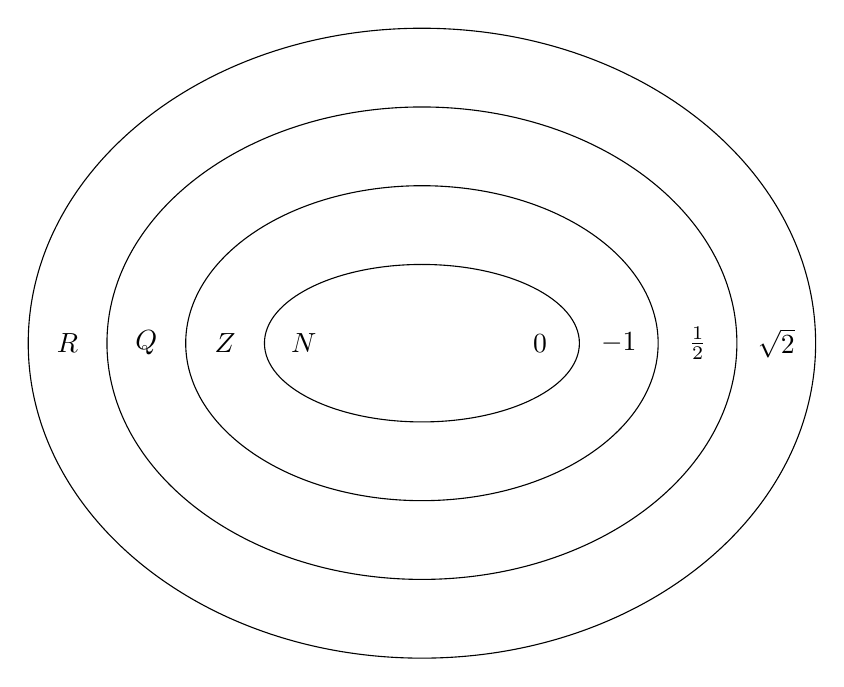
\begin{tikzpicture}
            \draw (0,0) ellipse (2cm and 1cm);
            \node at (-1.5,0) {\(\mathbb N\)};
            \node at (1.5,0) {\(0\)};
    
            \draw (0,0) ellipse (3cm and 2cm);
            \node at (-2.5,0) {\(\mathbb Z\)};
            \node at (2.5,0) {\(-1\)};
    
            \draw (0,0) ellipse (4cm and 3cm);
            \node at (-3.5,0) {\(\mathbb Q\)};
            \node at (3.5,0) {\(\frac{1}{2}\)};
    
            \draw (0,0) ellipse (5cm and 4cm);
            \node at (-4.5,0) {\(\mathbb R\)};
            \node at (4.5,0) {\(\sqrt{2}\)};
        \end{tikzpicture}
    \end{center}
    \caption[short]{Die grundlegenden Zahlenmengen sind ineinander enthalten.}
\end{figure}

\subsection{Die natürlichen Zahlen \(\mathbb N\)}
\begin{definition}[Menge der natürlichen Zahlen]
    \begin{equation*}
        \mathbb N := \{0,1,2,3,4,\dots\}
    \end{equation*}
\end{definition}
Können wir in den natürlichen Zahlen addieren? => Ja

Können wir subtrahieren? => Nein! Denn \(0 - 1 = -1 \notin \mathbb N\). 

\subsection{Die ganzen Zahlen \(\mathbb Z\)}
\begin{definition}[Menge der ganzen Zahlen]
    \begin{equation*}
        \mathbb Z := \{-n \mid n \in \mathbb N\} \cup \mathbb N
    \end{equation*}
\end{definition}
Der Satz vom Nullprodukt (\(\mathbb Z\) als Integritätsbereich, d.h. ohne Nullteiler -> Warum ist das nicht selbstverständlich -> Exkurs: Restklassenringe)

\begin{theorem}[Satz vom Nullprodukt]
    Keine Nullteiler
\end{theorem}

Können wir addieren? Ja. Können wir subtrahieren? Ja. Können wir multiplizieren? Ja. Können wir dividieren, d.h. teilen? Fast => Division mit Rest. 

\begin{theorem}[Division mit Rest]
    Division mit Rest => Problem: Es gibt Reste, d.h. nicht genaue Teiler!
\end{theorem}

\begin{definition}[Teiler einer ganzen Zahl]
    
\end{definition}

\begin{definition}[Primzahl]
    
\end{definition}

Warum sind Primzahlen besonders? Weil sie auf eine bestimmte Art \textit{elementar} sind: Jede ganze Zahl lässt sich \textit{eindeutig} als Produkt von Primzahlen darstellen. 

\begin{theorem}[Eindeutige Primfaktorzerlegung]
    Primfaktorzerlegung! (v.a. formale Notation)
\end{theorem}

\subsection{Die rationalen Zahlen \(\mathbb Q\)}
\begin{definition}[Menge der rationalen Zahlen]
    \begin{equation*}
        \mathbb Q := \left\{\frac{a}{b}\mid a \in \mathbb Z, b \in \mathbb N_{\geq 1}\right\}
    \end{equation*}
\end{definition}

Können wir addieren? Ja. Können wir subtrahieren? Ja. Können wir multiplizieren? Ja. Können wir dividieren, d.h. teilen? Ja!

\subsection{Die reellen Zahlen \(\mathbb R\)}
Irrationale Zahlen: Berühmter Irrationalitätsbeweis von Euklid von \(\sqrt{2}\). 

Können wir addieren? Ja. Können wir subtrahieren? Ja. Können wir multiplizieren? Ja. Können wir dividieren, d.h. teilen? Ja!

\begin{definition}[(Quadrat-, Kubik-)Wurzeln, Radikanten]
    Sei \(r \in \mathbb R\) und \( n \in \mathbb N_{\geq 1}\) ein Exponent. Dann heißt die reelle Zahl \(w \in \mathbb R, w>0\) für die gilt 
    \begin{equation*}
        w^n = r
    \end{equation*}
    \(n\)-te \textbf{Wurzel} von \(r\). Im Fall \(n=2\) sprechen wir auch von \textbf{Quadratwurzeln} und für \(n=3\) von \textbf{Kubikwurzeln}. Ist \(w\) die \(n\)-te Wurzel von \(r\), so schreiben wir \(w = \sqrt[n]{r}\). Ferner nennen wir dann \(r\) \textbf{Radikant} der Wurzel \(w\).  
\end{definition}
Wir kennen bereits einige Wurzeln aus der Grundschule. Zum Beispiel gilt \(5^2 = 25\). Also ist \(5\) die Quadratwurzel von \(25\) und \(25\) der Radikant von \(\sqrt{25}=5\). Eine weitere bekannte Quadratwurzel ist die Diagonallänge des Einheitsquadrats: \(\sqrt{2}\). Diese Quadratwurzel ist zusätzlich interessant, da sie irrational ist, also \(\sqrt{2}\notin \mathbb Q\) gilt. Diese Tatsache hatte bereits Euklid durch einen Widerspruch zeigen können: 

\begin{theorem}\label{thm:quadratwurzel-2-irrational}
    Die Quadratwurzel von \(2\) ist irrational. 
\end{theorem}
Bevor wir diesen Satz jedoch rigoros beweisen können, beweisen wir zunächst eine kleine Hilfsaussage.
\begin{lemma}\label{lem:primteiler-von-quadraten}
    Sei \(a \in \mathbb Z\). Ist \(p \in \mathbb Z\) ein Primteiler von \(a^2\), d.h. \(p\) prim und \(p\) teilt \(a^2\), so ist \(p\) auch ein Teiler von \(a\). 
\end{lemma}
\begin{proof}
    Dass \(p\) ein Teiler von \(a^2\) ist, bedeutet, dass ein \(m \in \mathbb Z\) existiert mit \(p \cdot m = a^2 = a\cdot a\). Mit der eindeutigen Primfaktorzerlegung folgt, dass \(p\) ein Primfaktor von \(a\) ist: Wir können \(a\) in seine \textit{eindeutigen} Primfaktoren zerlegen. Dadurch erhalten wir die eindeutige Zerlegung von \(a^2\). Genauer: Sei \(a = \prod_{i=1}^n p_i^{e_i}\) die eindeutige Primfaktorzerlegung von \(a\). Dann ist 
    \begin{equation*}
        a^2 = \left(\prod_{i=1}^n p_i^{e_i}\right)^2 = \prod_{i=1}^n (p_i^{e_i})^2 = \prod_{i=1}^n p_i^{2\cdot e_i}
    \end{equation*}
    Wir haben also eine Primfaktorzerlegung von \(a^2\) gefunden. Da Primfaktorzerlegungen eindeutig sind, haben wir \textit{die} Primfaktorzerlegung von \(a^2\) gefunden. Unser vorausgesetzter Primteiler muss also einer dieser Faktoren sein. Es gibt also ein \(j\), sodass \(p = p_j\). Damit ist \(p\) auch ein Primfaktor von \(a\). In anderen Worten: \(p\) teilt \(a\). 
\end{proof}
\begin{example}
    Ein "`Gegenbeispiel"' für die obige Aussage ist das folgende: \(25\) teilt \(100\), denn \(4\cdot 25 = 100\). Weiter gilt \(100 = 10^2\). Allerdings teilt \(25\) nicht \(10\). Das ist kein Widerspruch zum vorausgegangenen Lemma, da \(\sqrt{25} = 5 \cdot 5\), wir aber im Lemma verlangen, dass \(25\) eine Primzahl ist. Also können wir das Lemma hier nicht anwenden. 
\end{example}
Ausgerüstet mit dieser Hilfsaussage können wir den Euklidschen Widerspruchsbeweis rigoros führen. 

\begin{proof}[Beweis von Satz \ref{thm:quadratwurzel-2-irrational}]
    Wir führen einen Widerspruchsbeweis. Wir nehmen also an, dass \(\sqrt{2}\) rational wäre. Dann existieren \(a \in \mathbb Z, b \in \mathbb N_{\geq 1}\), sodass \(\left(\frac{a}{b}\right)^2 = 2\). Indem wir den Bruch soweit kürzen, dass wir nicht weiter kürzen können, erhalten wir \(r \in \mathbb Z, s \in \mathbb N_{\geq 1}\), sodass 
    \begin{equation}\label{eq:sqrt-2-beweis-1}
        \left(\frac{r}{s}\right)^2 = 2
    \end{equation}
    Dass wir nicht weiter kürzen können, bedeutet, dass \(r\) und \(s\) keine \textit{gemeinsamen Teiler} mehr haben. Denn sonst könnten wir diese ausklammern und weiter kürzen. Wir sprechen hierbei auch davon, dass \(r\) und \(s\) \textit{teilerfremd} sind. Darauf wird unser Widerspruch aufbauen. 

    Indem wir beide Seiten der Gleichung \eqref{eq:sqrt-2-beweis-1} mit \(s^2\) multiplizieren, erhalten wir \(r^2 = 2s^2\). Damit ist \(r^2\) durch \(2\) teilbar. Jetzt kommt unsere Hilfsaussage ins Spiel: \(2\) ist eine Primzahl und teilt \(r^2\) und \(r \in \mathbb Z\). Damit liefert \cref{lem:primteiler-von-quadraten}, dass \(2\) auch \(r\) teilt. Es existiert also ein \(t \in \mathbb Z\), sodass \(r = 2t\). Einsetzen in \(r^2 = 2s^2\) liefert \(4t^2 = 2s^2\) und damit \(s^2 = 2t^2\). Also ist \(2\) ein Teiler von \(s^2\). Wieder können wir \cref{lem:primteiler-von-quadraten} anwenden und erhalten, dass \(2\) auch \(s\) teilt. 

    Insgesamt haben wir also, dass \(2\) sowohl \(r\), als auch \(s\) teilt. In anderen Worten: \(2\) ist ein gemeinsamer Teiler von \(r\) und \(s\). Wir hatten jedoch \(r\) und \(s\) so gebaut, dass sie \textit{keine} gemeinsamen Teiler haben. Also haben wir einen Widerspruch gefunden. 
\end{proof}

Natürlich hatte Euklid diesen Beweis zu seiner Zeit nicht in dieser formellen Sprache formuliert, die wir heute verwenden. Viel eher hatte er über diese Aussage geometrisch nachgedacht. Denn dank dem Satz des Pythagoras war bereits lange vor Euklid bekannt, dass für die Länge \(d\) der Diagonalen im Einheitsquadrat (Abbildung) gilt 

\begin{equation*}
    d^2 = 1^2 + 1^2 = 2 
\end{equation*}

\begin{figure}
    % height "fix": https://stackoverflow.com/questions/56068071/large-bottom-margin-when-wrapping-text-around-the-image
    \begin{center}
        \begin{tikzpicture}
            \draw (0,0) rectangle (3,3);
            \node[anchor=west] at (3,1.5) {1};
            \node[anchor=north] at (1.5,0) {1};
        
            \draw[dashed] (0,0) -- (3,3) node[pos=.5, anchor=south east] {\(\sqrt{2}\)};
        \end{tikzpicture}
    \end{center}
    \caption[short]{Die Diagonale im Einheitsquadrat hat die Länge \(\sqrt{2}\).}
\end{figure}

Existiert zu jeder reellen Zahl eine \(n\)-te Wurzel? Ist \(n\) gerade, also z.B. \(n=2\), so gilt \(\sqrt{-1} \notin \mathbb R\). Allgemein gilt für jede reelle Zahl \(r \in \mathbb R_{>0}\), dass \(\sqrt{-r}\notin \mathbb R\) - Also in Worten: \(-r\) hat keine Quadratwurzel in \(\mathbb R\). Denn dafür müsste \((\sqrt{-r})^2 = -r <0\) gelten. Allerdings ist das Quadrat jeder reellen Zahl positiv\footnote{Das sieht man leicht durch eine Fallunterscheidung: Sei \(r \in \mathbb R, r \neq 0\). Ist \(r>0\), so gilt auch \(r^2\)>0. Ist \(r<0\), setzen wir \(p := -r\). Dann gilt insbesondere \(p>0\) und \(r = -p\). Es folgt \(r^2 = r\cdot r = (-p)\cdot (-p) = ((-1)\cdot p)((-1)\cdot p) = (-1)(-1)\cdot p\cdot p = p^2>0\).}, also auch \((\sqrt{-r})^2 \geq 0\). 

\begin{proposition}
    Für gerade \(n\)-te Wurzeln, d.h. \(n = 2m\) für ein \(m \in \mathbb N\) gilt 
    \begin{equation*}
        \sqrt[n]{r^n} = |r|
    \end{equation*}
    für alle \(r \in \mathbb R\). Insbesondere gilt \(\sqrt{(-r)^2}=|-r| = r\).
\end{proposition}
\begin{proof}
    Die Aussage gilt per Definition: In Definition (...) haben wir gerade Wurzeln als positive Werte definiert. Warum? Damit wir Wurzelfunktionen als Funktionen betrachten können. Sonst gäbe es nämlich immer zwei gerade Wurzeln! Haben wir eine, so ist deren Negatives ebenfalls eine valide Wurzel. Konkret: Hier ist sowohl \(r^n = r^n\) -- also könnten wir auch \(\sqrt[n]{r^n} = r\) schreiben, sofern wir das Vorzeichen ignorieren --, als auch \((-r)^n = (-r)^{2m} = (-1)^{2m}\cdot r^{2m} = r^{n}\) -- also auch \(\sqrt[n]{r^n} = -r\). Siehe auch \href{https://math.stackexchange.com/a/258880}{Math StackExchange}.
\end{proof}

Welche Gleichungen kann man in den reellen Zahlen noch nicht lösen? Alles mit negativen Radikanten! => Komplexe Zahlen (Exkurs). 

\section{Teilbarkeit und Primzahlen}

\section{Die binomischen Formeln}

\begin{theorem}[Binomischer Lehrsatz]
    Für eine Potenz \(n \in \mathbb N\) und \(a,b \in \mathbb R\) gilt 
    \begin{equation*}
        (a+b)^n = \sum_{k=0}^n \binom{n}{k}a^k b^{n-k}
    \end{equation*}
\end{theorem}

\section{Unendlichkeiten (*)}

\section{Grenzwerte (*)}